\documentclass[letterpaper,8pt,twocolumn,twoside,]{pinp}

%% Some pieces required from the pandoc template
\providecommand{\tightlist}{%
  \setlength{\itemsep}{0pt}\setlength{\parskip}{0pt}}

% Use the lineno option to display guide line numbers if required.
% Note that the use of elements such as single-column equations
% may affect the guide line number alignment.

\usepackage[T1]{fontenc}
\usepackage[utf8]{inputenc}

% pinp change: the geometry package layout settings need to be set here, not in pinp.cls
\geometry{layoutsize={0.95588\paperwidth,0.98864\paperheight},%
  layouthoffset=0.02206\paperwidth, layoutvoffset=0.00568\paperheight}

\definecolor{pinpblue}{HTML}{185FAF}  % imagecolorpicker on blue for new R logo
\definecolor{pnasbluetext}{RGB}{101,0,0} %



\title{PhD Proposal: Reservation Exchange and Dynamic Pricing \&
Procurement}

\author[a]{Edward Jie Xu}

  \affil[a]{Department of Technology, Management and Economics,
Technical Univeristy of Denmark, Denmark}

\setcounter{secnumdepth}{5}

% Please give the surname of the lead author for the running footer
\leadauthor{}

% Keywords are not mandatory, but authors are strongly encouraged to provide them. If provided, please include two to five keywords, separated by the pipe symbol, e.g:
 

\begin{abstract}
Highlights: @ A continuous double auction market with a new type of
limit order books is proposed to replace incumbent electricity families,
making it possible for small-scale prosumers to directly participate. @
Discrete event simulations of multi-agent systems are used as the main
research tools to demonstrate market operations and decision-making
processes. @ A new decision-making framework based on model predictive
control is introduced to facilitate procurement, control and response of
participants. @ Based on the same idea, a business as retailers can be
started up in incumbent power industries as real-world experiments.
Existing literature in revenue management, inventory management, supply
chain management, etc can be put into use. @ Simulations can provide
statistics for long-term investments, and a new structure for power
systems can emerge, especially in underdeveloped areas. @ The market can
be applied in other industries, like food supply chains, the retailing
and the banking.
\end{abstract}

\dates{This version was compiled on \today} 

% initially we use doi so keep for backwards compatibility
% new name is doi_footer


\begin{document}

% Optional adjustment to line up main text (after abstract) of first page with line numbers, when using both lineno and twocolumn options.
% You should only change this length when you've finalised the article contents.
\verticaladjustment{-2pt}

\maketitle
\thispagestyle{firststyle}
\ifthenelse{\boolean{shortarticle}}{\ifthenelse{\boolean{singlecolumn}}{\abscontentformatted}{\abscontent}}{}

% If your first paragraph (i.e. with the \dropcap) contains a list environment (quote, quotation, theorem, definition, enumerate, itemize...), the line after the list may have some extra indentation. If this is the case, add \parshape=0 to the end of the list environment.


\hypertarget{aim-and-novelty}{%
\section{Aim and Novelty}\label{aim-and-novelty}}

In the power industry, it is urgent to reduce the carbon emission from
power generations, avoid backup generators and penetrate modern power
systems. Other industries, like food supply chains, face similar
challenges. The lack of direct participation from the demand side is the
central question, which may be solved by the market designed in the
project. Arguments for these designs can be established in two stages:

\begin{itemize}
\tightlist
\item
  Because of the complexity, in the first stage, simulations instead of
  analysis are primarily used to demonstrate how the market operates and
  prosumers make decisions under different settings. To facilitate the
  simulation of participants in the market, a new decision-making
  framework is defined. The objective is to establish the most realistic
  simulation toolbox by trying candidate models and conducting computer
  experiments.
\item
  In the second stage, a new retailing business with similar features
  can be set up and field-tested in incumbent power systems, of which
  the results can be used to examine key assumptions and calibrate
  simulation models. With validated simulation models, new structures
  for power systems can be proposed.
\end{itemize}

The necessity for the new market is discussed in section
\ref{motivation}, followed by the description of the market in section
\ref{Rex}. The methodology is discussed in four parts of section
\ref{method}. The first part introduces the simulation schemes used, and
the second part discusses the core simulation programs. The project can
be researched from three perspectives, which are listed in the third
part, and the most important one is elaborated in the last part.
Expected contributions are summarized in the last section.

\hypertarget{background-and-motivation}{%
\section{Background and Motivation}\label{background-and-motivation}}

\label{motivation}

Small-scale producers/consumers (\textbf{prosumers})
\protect\hyperlink{reference}{parag2016electricity} prefer entering into
contracts to isolate themselves from the vagaries of wholesale markets,
so their participation is mediated by retailers, who take the risk and
profit from premiums. This strategy is widely applied in industries with
durables, while is impractical for fresh foods and electricity because
of their continuous generations/consumptions, reliance on
\textbf{delivery networks}, and time-dependence. Retailers must face
price spikes from time to time because they are obliged to satisfy the
needs of their customers.
\protect\hyperlink{reference}{kirschen2003demand}

Instead, mechanisms satisfying the following requirements should be
applied:

\begin{itemize}
\tightlist
\item
  Adaptive to external factors temporally and spatially. For example,
  time-varying peak loads resulted from penetration of renewable
  generations exclude applications of traditional load shifting or
  shedding. \protect\hyperlink{reference}{connell2014benefits}
\item
  The market should be as transparent as possible, while private
  information is tightly protected. Neither centralized
  command-and-control nor retailing is efficient in such settings
  because of the conflict between better market clearings and
  information protection.
  \protect\hyperlink{reference}{kirschen2018fundamentals} It is
  prosumers who anticipate their future states, formulate trading
  strategies and act accordingly.
\item
  Low-cost. Coordinated demand response is essential to ensure the
  quality of energy supply when none of the advanced technologies, like
  large-scale storage, hydropower, nuclear power, can be relied on to
  balance power systems in underdeveloped areas.
  \protect\hyperlink{reference}{jacome2019power}
\item
  Purchases should be ahead of deliveries
  \protect\hyperlink{reference}{prasad2011advance}, because the spot
  selling season is infinitely small. The real-time incentives from spot
  markets are hard to catch, because not only the current signals can
  hardly reveal any information about the future, but also prosumers
  need time to adapt their activities to fit traded quantities.
  \protect\hyperlink{reference}{kirschen2000factoring}
\item
  Transactions can be instantaneous because some prosumers arrive
  randomly and may demand liquidity.
  \protect\hyperlink{reference}{foucault2013market} Also, some would
  like to trade for long periods covering many trading units to save the
  trouble from making decisions regarding few units but in high
  frequency.
\item
  The market is thick enough but not congested, so prosumers do not have
  to search or bargain. In other words, the market is liquid enough for
  prosumers to lower transaction costs.
\item
  The number of statistics for decision making is as low as possible but
  different assets can be distinguished based on those statistics.
\item
  The imbalance within trading units can be maintained without
  centralized system operators
  \protect\hyperlink{reference}{kirschen2018fundamentals}, because it
  may be hard to establish trustworthy regulatory authorities and
  operators responsible for the system safety.
\end{itemize}

Till now, all market designs fail to fulfil these requirements, while in
this project, at least one capable market is brought up. The most
promising candidate so far is introduced in section \ref{Rex}, following
discussions about its primary function, traded assets, two features, and
superiority over others.

\hypertarget{proposed-solution-reservation-exchange}{%
\section{Proposed Solution: Reservation
Exchange}\label{proposed-solution-reservation-exchange}}

\label{Rex}

The proposed solution is a \textbf{continuous double auction} market
with \textbf{3-dimensional limit order books}, where prosumers can
bid/offer continuously and get transacted once matched with another
order. It allows immediate transactions and standby orders at the same
time. Similar to computerized reservation systems in airline industries,
prosumers have to book before the delivery, and markets are segmented
according to when bookings are made.
\protect\hyperlink{reference}{shy2008how} Therefore the market is named
\textbf{reservation exchange (Rex)}. With delivery networks integrated,
the whole system is named \textbf{RexNet}.
\footnote{Two names are used interchangeably.} For power industries, Rex
can be used to replace the market families including day-ahead market,
intra-day market, balancing market, capacity market and other ancillary
markets.

The most important function of Rex is \textbf{quantity discovery}, which
is similar to price discovery in limit order markets for financial
assets when markets motivate participants to reveal their private
valuations. \protect\hyperlink{reference}{maloney2003complexity} Two
kinds of discoveries can be generalized as dynamic equilibrium
discovery, which creates knowledge by incorporating dispersed
information at high speed.
\protect\hyperlink{reference}{birchler2007information} Likewise,
prosumers are encouraged to take advantage of their information about
the aggregated prosumptions in Rex, so mismatches can be eliminated in
high speed without the necessity for centralized monitoring.

Traded assets in Rex belong to \textbf{time-dependent products (TDP)}.
Different kinds of service always involve producers and consumers at the
same time, making it the majority of TDP. Some settings have been
introduced to convert electricity into tradable TDP and differentiate
them temporally and spatially.

In this project, all kinds of delivery networks can be divided into two
levels: distribution networks (whose constraints can be ignored) and
transmission networks. The market is \textbf{spatially fragmented} by
transmission networks when relevant edges are congested, so stakeholders
in control of transmission networks can participate in Rex as spatial
arbitragers. Moreover, Rex can be established \textbf{hierarchically}.
Representatives of prosumers in lower levels can serve as retailers,
which makes the experiments in subsection \ref{EXP} plausible.

Though the structure of Rex is similar to that composed of day-ahead
markets and intraday markets, the main difference is that there is no
one responsible for satisfying uninformed demand of prosumers in Rex.
For example, utility companies are not obliged to satisfy demand in peak
hours. If \textbf{reservation} and \textbf{realization} does not match,
he/she has to take the consequence. Thus, there is no need for
centralized managers to maintain system safety. So despite the
similarity, methods in \protect\hyperlink{reference}{nair2014energy} and
\protect\hyperlink{reference}{secomandi2014optimal} are fundamentally
different from those in this project.

Also, trading volumes in intraday markets are insignificant compared to
those in day-ahead markets and balancing markets
\protect\hyperlink{reference}{weber2010adequate}, so most of the current
researches focus on periodic double auctions used in day-ahead markets.
Approaches to Rex deviate from these researches, and decision-making
processes are different as well.

With only one type of agents (prosumers) providing and consuming
liquidity, Rex is an \textbf{order-driven continuous double auction
market} in essence. \protect\hyperlink{reference}{gould2013limit} There
are many variations like quote-driven markets, where market makers are
the primary source of liquidity. As discussed in section
\ref{motivation}, it may be hard for small-scale prosumers to
participate if the market is not the most simple and flexible one,
making Rex the focus in the simulation stage. With adequate data and
assumptions validated in the second stage, better options may be
identified.

\hypertarget{methodology}{%
\section{Methodology}\label{methodology}}

\label{method}

Models and methods in the simulation stage will be elaborated first in
subsection \ref{DES}, then the decision making framework of prosumers is
introduced in subsection \ref{RHPO}. Some specific simulation programs
are presented as well. In subsection \ref{three}, three different ways
to analyze Rex are discussed. Finally, field experiments in the second
stage are outlined in subsection \ref{EXP}, and some key differences
from models in the literature are emphasized.

\hypertarget{first-stage-discrete-event-simulation-of-multi-agent-systems}{%
\subsection{First Stage: Discrete Event Simulation of Multi-Agent
Systems}\label{first-stage-discrete-event-simulation-of-multi-agent-systems}}

\label{DES}

Take energy systems, especially power systems, for example, they can be
represented by the figure \ref{1}-a, summarizing the supply chain from
extractions to end-uses, of which the key stage is the distribution from
the supply side to the demand side.
\protect\hyperlink{reference}{blok2017introduction} Alternatively, the
system can be restructured by figure \ref{1}-b by introducing Rex.
Prosumers can be modelled as three parts.

\begin{itemize}
\tightlist
\item
  \textbf{Clients} are used to simulate the ultimate needs of the
  prosumer like minimum requirements of room temperature in winter. They
  are assumed to report their forecasts unreservedly, despite
  imprecision before the realization.
\item
  \textbf{Continuous provision plants (CPPs)} are underlying physical
  and/or economical systems with inputs (electricity, sunshine, water,
  etc) and outputs to meet the needs of clients. For example, it can be
  an electricity-driven heat pump and pipes for space heating. Usually,
  there is inter-temporal dynamics within these systems, so the
  framework in subsection \ref{RHPO} is required.
\item
  It is \textbf{coordinators} who control CPPs and participate in Rex,
  and their objectives are to make more profit (or lower costs), satisfy
  needs and respect constraints at the same time. The direct
  participation of small-scale prosumers discussed in section
  \ref{motivation} is a critical premise for this structure so that
  there is no friction between these three parts because they refer to
  the same prosumer.
\end{itemize}

\begin{figure}
\centering
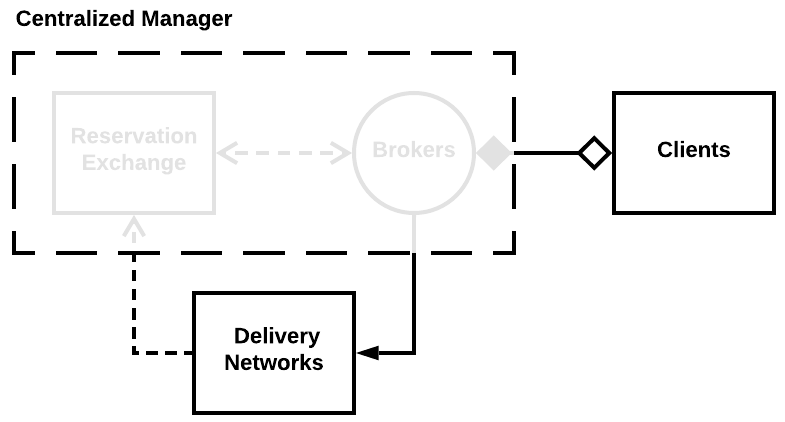
\includegraphics[width=0.48\textwidth]{../../../images/1-3.png}
\caption{Two ways to represent energy supply chains. (a) Illustration of energy supply chains. (b) Restructuring of the chains based on Rex.}
\label{1}
\end{figure}

In this project, we are interested in both the market and prosumers,
which therefore have to be modelled as \textbf{multi-agent systems},
because prosumers have diverging information and interests.
\protect\hyperlink{reference}{shoham2009multiagent} No centralized
manager knows all variable outcomes and controls everything, so the
market clearing process needs to be optimized in a distributed manner.
This structure distinguishes this project because researchers must model
heterogeneous prosumer instead of formulating a management strategy.

Hence, \textbf{agent-based models} are used
\protect\hyperlink{reference}{iori2012agent},
\protect\hyperlink{reference}{lebaron2001builder}, and their
interactions through Rex are demonstrated by \textbf{discrete event
simulations}.

\hypertarget{decision-making-framework-for-prosumers}{%
\subsection{Decision Making Framework for
Prosumers}\label{decision-making-framework-for-prosumers}}

\label{RHPO}

The simulation timeline can be summarized as follows. Some clients, like
wind turbines in power systems, are endowed with prosumptions, the
quantity of which are simulated with similar patterns to historical
data. Because they don't know the precise quantity in advance, they will
forecast based on their private up-to-date information, the outcomes of
which are simulated as well. Once their forecasts update, they will
convey the differences to coordinators, who are obliged to react to it
before gate closures. For the sake of privacy protections,
high-resolution models of CPPs are known to corresponding coordinators
only. Future outputs can be predicted from CPP models and planned
inputs. Then, coordinators modify plans, participate in Rex and
cooperate with clients.

The decisions can be optimized by \textbf{receding horizon plan \& order
management (RHPO)}, which has similar structures to model predictive
control problems. \protect\hyperlink{reference}{rawlings2019model} After
deciding trading volumes, coordinators have to manage \textbf{make-take
decisions} according to order flows, states of limit order books,
\protect\hyperlink{reference}{foucault2013market} and their private
evaluations of their positions. \textbf{Position} is the difference
between the market total volume and fundamental volume. The precision of
evaluations differs among prosumer., so quantities are discovered
because informed prosumers communicate their high-value information by
trading aggressively. Overall, the states of Rex are changed
instantaneously at separate time points when some coordinator submits
order according to its RHPO instructions, making the discrete event
simulation a reliable method.

Here are some prototypical stochastic simulation programs used in this
project:

\begin{itemize}
\tightlist
\item
  To simulate realizations, like those from wind turbines, at new
  locations according to historical data, statistical methods in the
  frequency domain can be utilized to exhibit the spatial diversity and
  make use of available information as much as possible.
  \protect\hyperlink{reference}{woods2013simulation}
\item
  To simulate evolutions of discrete states in a bottom-up way,
  inhomogeneous Markov chains can be constructed using detailed survey
  data. \protect\hyperlink{reference}{page2008generalised} For example,
  electricity consumptions of residents associated with their occupant
  presences can be obtained.
\item
  Martingale models of forecast evolution can be used to simulate
  requests sent to coordinators.
  \protect\hyperlink{reference}{heath1994modeling}
\item
  CPPs may correlate with each other so they must be modelled by an
  aggregated CPPs controlled by one coordinator to satisfy several
  clients. For example, the space heating system for multi-dwelling
  buildings must be modelled by multi-input-multi-output control
  systems. \protect\hyperlink{reference}{siroky2011experimental}
  Moreover, retailers can be introduced to form a hierarchical Rex,
  which will be discussed in subsection \ref{EXP}.
\item
  Grey-box modelling techniques, which combine statistical methods and
  physical knowledge, can be used to identify CPP models.
  \protect\hyperlink{reference}{bacher2011identifying}
\end{itemize}

\hypertarget{three-ways-to-analyze-rex}{%
\subsection{Three Ways to Analyze Rex}\label{three-ways-to-analyze-rex}}

\label{three}

There are three angles to this multi-agent system, which are illustrated
by figure \ref{2}.

\begin{itemize}
\tightlist
\item
  The first one is from coordinators, and it includes three elements for
  prosumers like those in two solid blue boxes.
\item
  The second one is to focus on the evolution of Rex and it includes
  coordinators only, which is shown by the dashed red box. The induction
  of stylized facts of Rex is the primary task, which makes it possible
  to simulate the market directly.
  \protect\hyperlink{reference}{buchanan2011it} Then the effect of
  different resolution parameters, introductions of market makers,
  replacement with periodic double auctions, etc may be explored. It
  also provides opportunities for researchers with the first perspective
  to tune parameters.
\item
  Last but not least, a holistic view including all models is necessary,
  because key features of Rex, like the shift from quantity-based to
  power-time-based cost allocation
  \protect\hyperlink{reference}{hougaard2009introduction}, must be
  examined this way. The quantity discovery function must be
  demonstrated in this way as well.
\end{itemize}

\begin{figure}
\begin{center}
  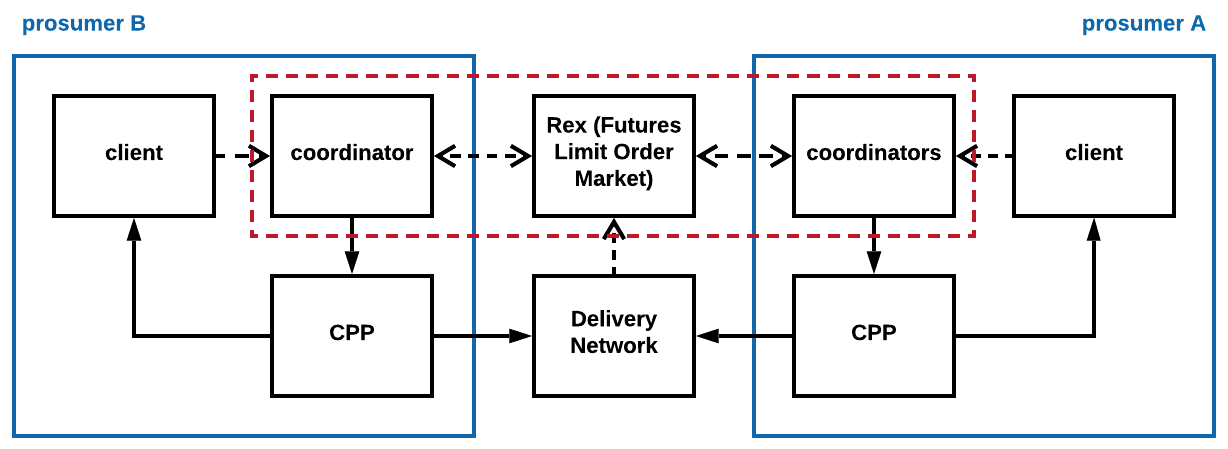
\includegraphics[width=0.48\textwidth]{../../../images/4-10.png}
\end{center}
\caption{Illustration of three ways to analyze Rex}
\label{2}
\end{figure}

\hypertarget{second-stage-dynamic-pricing-procurement}{%
\subsection{Second Stage: Dynamic Pricing \&
Procurement}\label{second-stage-dynamic-pricing-procurement}}

\label{EXP}

New business as retailers in incumbent power systems can be field-tested
in the second stage. As discussed in section \ref{Rex}, Rex can be
established in a hierarchical structure, so retailers can be introduced
to as another layer between prosumers and the market, which is
illustrated by figure \ref{3}. Prosumers still need to reserve via the
retailer instead of Rex. In this setting, retailers face a
\textbf{continuous forward dynamic pricing \& procurement (CFDPP)}
problem. The implementation of the retailing business and the analysis
of customer behaviours are the primary concern, so there is no need to
establish the whole market.

\begin{figure}
  \begin{center}
    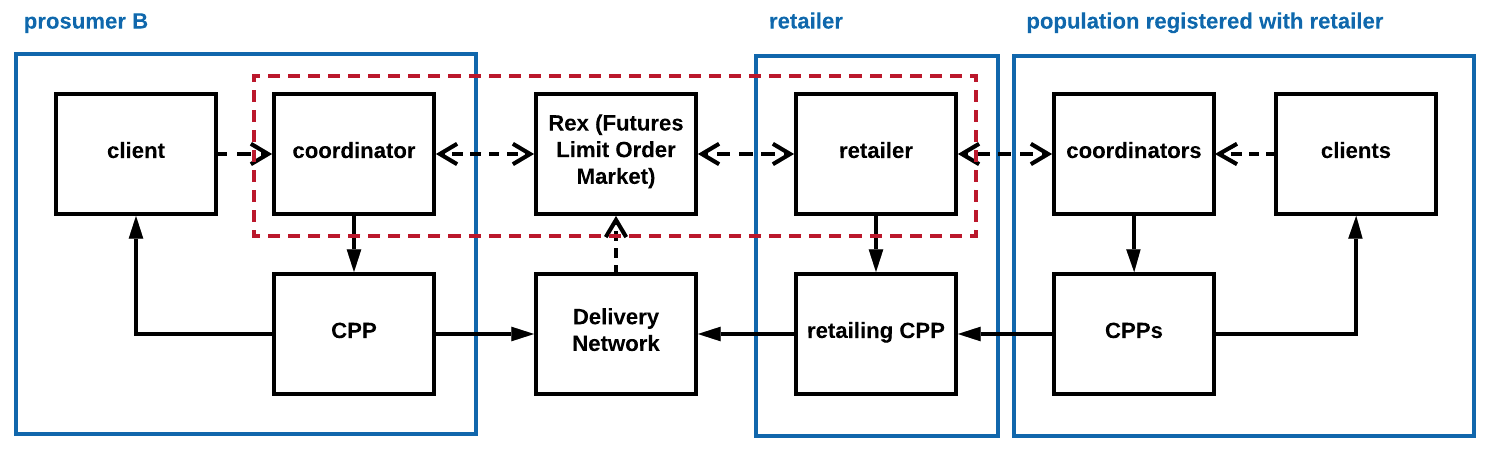
\includegraphics[width=0.46\textwidth]{../../../images/4-11.png}
  \end{center}
  \caption{Illustration of new businesss as retailers incumbent power systems}
  \label{3}
\end{figure}

Lots of existing literature can provide insights into CFDPP:

\begin{itemize}
\tightlist
\item
  Newsvendor's procurement.
  \protect\hyperlink{reference}{qin2011newsvendor} Dynamic procurement
  can be utlized when there are multiple decision epochs.
  \protect\hyperlink{reference}{wang2012multiordering}
\item
  Forward dynamic pricing of TDP. The initial inventory is endowed
  without cost considered in contrast to that in the previous category.
  Most of the techniques are from revenue management.
  \protect\hyperlink{reference}{gallego2019revenue}
\item
  Inventory management of perishables.
  \protect\hyperlink{reference}{nahmias2011perishable}
\item
  Dynamic pricing of durables.
  \protect\hyperlink{reference}{ahn2007pricing} When strategic
  behaviours of customers are endogenous, game theoretical models should
  be used. \protect\hyperlink{reference}{su2010intertemporal}
\item
  Advance selling from the perspective of retailers and reservation
  (booking) from the perspective of customers.
  \protect\hyperlink{reference}{shugan2000advance} Much literature
  focuses on how to deal with strategic customers.
  \protect\hyperlink{reference}{prasad2011advance},
  \protect\hyperlink{reference}{zhao2010pre}
\end{itemize}

Essential terminologies from the above literature are illustrated using
figure \ref{4}. There are some highlights:

\begin{itemize}
\tightlist
\item
  Prosumers do not know about their endowments or utilities for sure at
  reservation decision epochs.
  \protect\hyperlink{reference}{shugan2000advance}
\item
  Regarding demand, the conservative approach is to assume that it is
  either satisfied (leading to sales) or lost forever, and there is only
  one product in the market.
  \protect\hyperlink{reference}{shen2007customer} Instead, a continuous
  manner must be adopted to tackle inter-temporal decisions, for which
  RHPOs are designed.
\item
  Outcomes of random variables are always assumed to be known to
  everyone immediately in existing literature
  \protect\hyperlink{reference}{su2010optimal}, ignoring the discovery
  process.
\item
  Procurement costs in future epochs are stochastic.
\end{itemize}

\begin{figure}
\begin{center}
  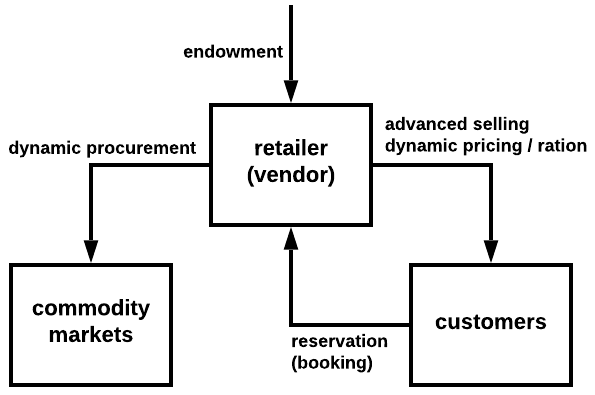
\includegraphics[width=0.40\textwidth]{../../../images/4-12.png}
\end{center}
\caption{Illustration of the new businesss using terminologies from relevant literature.}
\label{4}
\end{figure}

Key assumptions in simulation programs can be evaluated using the
experiment results. Besides, it is vital to validate simulation programs
based on measured data.
\protect\hyperlink{reference}{ross2012simulation} For example, simulated
forecast evolution should be analyzed according to standard analytical
tools for forecasting
\protect\hyperlink{reference}{madsen2005standardizing} and compared to
results from state-of-art forecast techniques.

\hypertarget{expected-contributions}{%
\section{Expected Contributions}\label{expected-contributions}}

The assumption of time invariance can be relaxed once short-term models
are mature. The existence of investments, ageing and accidents brings
about more randomness and flexibility.
\protect\hyperlink{reference}{spyrou2019planning} Usually, massive
long-term infrastructure investment is required in power industries.
Simulation results from Rex indicate investment opportunities. The
ultimate goal of this project is to formulate a new structure for
resilient, low-carbon, low-cost energy systems based on Rex.

With simulation methods validated, Rex can be applied in other
industries like food supply chains, retailing, banking, etc. Besides,
similar assets can still be pooled, when personalized limit order books
are introduced to find matches with requirements satisfied from both
sides. The process is similar to that in peer-to-peer markets with
bilateral trade agreements. \protect\hyperlink{reference}{sousa2019peer}

All in all, following problems are expected to be solved:

\begin{itemize}
\tightlist
\item
  The effect of reservations on responsive clients, who can adapt their
  needs to current states, is not clear. It may be modelled by an
  intra-personal game where a decision-maker is summarized by a
  succession of selves \protect\hyperlink{reference}{brocas2009dynamic}
  or joint workings of time inconsistency \& consciousness.
  \protect\hyperlink{reference}{birchler2007information}
\item
  When optimization problems in RHPO are formulated nonlinearly, it may
  be hard to obtain shadow prices, which indicate costs of flexibility
  and responsiveness.
\item
  Agent-based models should be able to learn and adapt to evolving
  situations. \protect\hyperlink{reference}{franklin1997it}
\item
  The determination of weight matrices is the challenge faced by MPC
  researchers as well \protect\hyperlink{reference}{rawlings2019model},
  and the tuning relies heavily on methods discussed in subsection
  \ref{three}.
\item
  How to make Rex robust to external factors.
\end{itemize}

As discussed above, the project can be divided into two stages. Expected
outputs of simulation experiments in the first stage are:

\begin{itemize}
\tightlist
\item
  Introduction to Rex. (my DTU master thesis)
\item
  RHPO for more complex CPPs, like those with stochastic MIMOs, and
  their statistical identification methods.
\item
  Rex with responsive clients.
\end{itemize}

\hypertarget{reference}{%
\section{Reference}\label{reference}}

\begin{itemize}
\tightlist
\item
  \href{https://www.sciencedirect.com/science/article/pii/S0378778811000491}{bacher2011identifying}
  Bacher, P., \& Madsen, H. (2011). Identifying suitable models for the
  heat dynamics of buildings. Energy and Buildings, 43(7), 1511-1522.
\item
  \href{https://www.taylorfrancis.com/books/9780203946558}{birchler2007information}
  Birchler, U., \& Bütler, M. (1999). Information economics. Routledge.
  \emph{How the market aggregates information is discussed in 5 chapters
  in part 2. All kinds of deviations of behaviours by later self are
  introduced briefly in chapter 17.}
\item
  \href{https://www.taylorfrancis.com/books/9781315617213}{blok2017introduction}
  Blok, K., \& Nieuwlaar, E. (2016). Introduction to energy analysis.
  Taylor \& Francis. \emph{Figure \texttt{a} is the figure 0.1 on page
  xxv.}
\item
  \href{https://link.springer.com/article/10.1007/s11238-009-9183-x}{brocas2009dynamic}
  Brocas, I. (2011). Dynamic inconsistency and choice. Theory and
  decision, 71(3), 343-364.
\item
  \href{https://www.nature.com/articles/nphys2191}{buchanan2011it}
  Buchanan, M. (2012). It's a (stylized) fact!. Nature Physics, 8(1),
  3-3.
\item
  \href{https://www.sciencedirect.com/science/article/pii/S1364032114005504}{connell2014benefits}
  Pinson, P., \& Madsen, H. (2014). Benefits and challenges of
  electrical demand response: A critical review. Renewable and
  Sustainable Energy Reviews, 39, 686-699. \emph{In section 1-2, the
  necessity of continuous demand response is discussed.}
\item
  \href{https://www.oxfordscholarship.com/view/10.1093/acprof:oso/9780199936243.001.0001/acprof-9780199936243}{foucault2013market}
  Foucault, T., Pagano, M., Roell, A., \& Röell, A. (2013). Market
  liquidity: theory, evidence, and policy. Oxford University Press.
  \emph{How real-world markets work is introduced at the beginning of
  chapter 1. Make- and Take- decisions in LOB markets are discussed in
  chapter 6.}
\item
  \href{https://link.springer.com/chapter/10.1007/BFb0013570}{franklin1997it}
  Franklin, S., \& Graesser, A. (1996, August). Is it an Agent, or just
  a Program?: A Taxonomy for Autonomous Agents. In International
  Workshop on Agent Theories, Architectures, and Languages (pp.~21-35).
  Springer, Berlin, Heidelberg.
\item
  \href{https://link.springer.com/book/10.1007/978-1-4939-9606-3}{gallego2019revenue}
  Gallego, G., \& Topaloglu, H. (2019). Revenue management and pricing
  analysis. Springer, New York.
\item
  \href{https://www.tandfonline.com/doi/abs/10.1080/14697688.2013.803148}{gould2013limit}
  Gould, M. D., Porter, M. A., Williams, S., McDonald, M., Fenn, D. J.,
  \& Howison, S. D. (2013). Limit order books. Quantitative Finance,
  13(11), 1709-1742.
\item
  \href{https://www.tandfonline.com/doi/abs/10.1080/07408179408966604}{heath1994modeling}
  Heath, D. C., \& Jackson, P. L. (1994). Modeling the evolution of
  demand forecasts ITH application to safety stock analysis in
  production/distribution systems. IIE transactions, 26(3), 17-30.
  \emph{MMFEs are not forecasting techniques, but programs to simulate
  the forecast results.}
\item
  \href{https://link.springer.com/book/10.1007/978-3-642-01828-2}{hougaard2009introduction}
  Hougaard, J. L. (2009). An introduction to allocation rules. Springer
  Science \& Business Media.
\item
  \href{https://www.oxfordhandbooks.com/view/10.1093/oxfordhb/9780199844371.001.0001/oxfordhb-9780199844371-e-43}{iori2012agent}
  Iori, G., \& Porter, J. (2012). Agent-based modelling for financial
  markets. Chapter prepared for the Handbook on Computational Economics
  and Finance. \emph{Section 4-2 is about heterogeneous agents with
  market mediated interactions.}
\item
  \href{https://www.pnas.org/content/116/33/16308}{jacome2019power}
  Jacome, V., Klugman, N., Wolfram, C., Grunfeld, B., Callaway, D., \&
  Ray, I. (2019). Power quality and modern energy for all. Proceedings
  of the National Academy of Sciences, 116(33), 16308-16313. \emph{The
  operation of power grids in less-developed areas is different from
  that in developed countries because the systems are not resilient
  enough for lack of responsive generators, large-scale connections,
  regulations, etc.}
\item
  \href{https://ieeexplore.ieee.org/document/867149}{kirschen2000factoring}
  Kirschen, D. S., Strbac, G., Cumperayot, P., \& de Paiva Mendes, D.
  (2000). Factoring the elasticity of demand in electricity prices. IEEE
  Transactions on Power Systems, 15(2), 612-617.
\item
  \href{https://ieeexplore.ieee.org/document/1198281}{kirschen2003demand}
  Kirschen, D. S. (2003). Demand-side view of electricity markets. IEEE
  Transactions on power systems, 18(2), 520-527. \emph{Price spikes in
  electricity markets are discussed in section 2.}
\item
  \href{https://www.wiley.com/en-us/Fundamentals+of+Power+System+Economics\%2C+2nd+Edition-p-9781119213253}{kirschen2018fundamentals}
  Kirschen, D. S., \& Strbac, G. (2018). Fundamentals of power system
  economics. John Wiley \& Sons. \emph{Issues associated with retailers
  are discussed in section 4-3, and those with centralized tradings are
  in section 3-3-3. Why and how centralized system operators in
  incumbent electricity markets maintain safety within trading units are
  discussed in chapter 6. However, system operators are expected to be
  eliminated in this project.}
\item
  \href{https://www.tandfonline.com/doi/abs/10.1088/1469-7688/1/2/307}{lebaron2001builder}
  LeBaron, B. (2001). A builder's guide to agent-based financial
  markets. Quantitative finance, 1(2), 254-261. \emph{``It is not really
  a survey, but a kind of view from the trenches in terms of building
  artificial markets.''}
\item
  \href{https://journals.sagepub.com/doi/abs/10.1260/030952405776234599}{madsen2005standardizing}
  Madsen, H., Pinson, P., Kariniotakis, G., Nielsen, H. A., \& Nielsen,
  T. S. (2005). Standardizing the Performance Evaluation of Short-Term
  Wind Power Prediction Models. Wind Engineering, 29(6), 475--489.
\item
  \href{https://www.sciencedirect.com/science/article/pii/S092911990200055X}{maloney2003complexity}
  Maloney, M. T., \& Mulherin, J. H. (2003). The complexity of price
  discovery in an efficient market: the stock market reaction to the
  Challenger crash. Journal of corporate finance, 9(4), 453-479.
  \emph{An empirical event study on how the new knowledge and its
  associated equilibrium price is discovered.}
\item
  \href{https://www.springer.com/gp/book/9781441979988}{nahmias2011perishable}
  Nahmias, S. (2011). Perishable inventory systems (Vol. 160). Springer
  Science \& Business Media.
\item
  \href{https://dl.acm.org/doi/10.1145/2591971.2591982}{nair2014energy}
  Nair, J., Adlakha, S., \& Wierman, A. (2014, June). Energy procurement
  strategies in the presence of intermittent sources. In The 2014 ACM
  international conference on Measurement and modeling of computer
  systems (pp.~85-97).
\item
  \href{https://www.sciencedirect.com/science/article/pii/S037877880700031X}{page2008generalised}
  Page, J., Robinson, D., Morel, N., \& Scartezzini, J. L. (2008). A
  generalised stochastic model for the simulation of occupant presence.
  Energy and buildings, 40(2), 83-98.
\item
  \href{https://www.nature.com/articles/nenergy201632}{parag2016electricity}
  Parag, Y., \& Sovacool, B. K. (2016). Electricity market design for
  the prosumer era. Nature energy, 1(4), 1-6.
\item
  \href{https://onlinelibrary.wiley.com/doi/abs/10.1111/j.1937-5956.2010.01133.x?casa_token=lVRyRU67RhMAAAAA:8Dj0zKFhuT8i_4hkKs0PDvKRC3RUMLWaJk_poEYL7Z9oYcOJVB4-ZsEuT18KN15fuZcrCWLtaAeNayg}{prasad2011advance}
  Prasad, A., Stecke, K. E., \& Zhao, X. (2011). Advance selling by a
  newsvendor retailer. Production and Operations Management, 20(1),
  129-142. \emph{Behaviors of customers are discussed in subsection 3.2}
\item
  \href{https://www.sciencedirect.com/science/article/pii/S0377221710008040}{qin2011newsvendor}
  Qin, Y., Wang, R., Vakharia, A. J., Chen, Y., \& Seref, M. M. (2011).
  The newsvendor problem: Review and directions for future research.
  European Journal of Operational Research, 213(2), 361-374.
\item
  \href{https://sites.engineering.ucsb.edu/~jbraw/mpc/}{rawlings2019model}
  Rawlings, J. B., Mayne, D. Q., \& Diehl, M. (2017). Model predictive
  control: theory, computation, and design (Vol. 2). Madison, WI: Nob
  Hill Publishing. \emph{MPC regulators are introduced in chapter 1.}
\item
  \href{https://www.elsevier.com/books/simulation/ross/978-0-12-415825-2}{ross2012simulation}
  Ross, S. (2012) Simulation. Academic Press.
\item
  \href{https://pubsonline.informs.org/doi/10.1287/msom.2013.0473}{secomandi2014optimal}
  Secomandi, N., \& Kekre, S. (2014). Optimal energy procurement in spot
  and forward markets. Manufacturing \& Service Operations Management,
  16(2), 270-282.
\item
  \href{https://onlinelibrary.wiley.com/doi/abs/10.1111/j.1937-5956.2007.tb00291.x}{shen2007customer}
  Shen, Z. J. M., \& Su, X. (2007). Customer behavior modeling in
  revenue management and auctions: A review and new research
  opportunities. Production and operations management, 16(6), 713-728.
  \emph{Inter-temporal substitutions are discussed in section 2-1.}
\item
  \href{https://www.cambridge.org/core/books/multiagent-systems/B11B69E0CB9032D6EC0A254F59922360}{shoham2009multiagent}
  Shoham, Y., \& Leyton-Brown, K. (2008). Multiagent systems:
  Algorithmic, game-theoretic, and logical foundations. Cambridge
  University Press. \emph{MASs with continuous double auctions are
  discussed in section 11-4.}
\item
  \href{https://journals.sagepub.com/doi/abs/10.1177/109467050023001?casa_token=nHdK2gtk0ZUAAAAA:JZm0jvC2O9C0qr7WPZZphEZINBT2hpYCLNSB5hykwAO1buCHLim0JzlleOeUOwCv0uIZWbmfE8vI}{shugan2000advance}
  Shugan, S. M., \& Xie, J. (2000). Advance pricing of services and
  other implications of separating purchase and consumption. Journal of
  Service Research, 2(3), 227-239. \emph{Elasticities are different
  regarding purchasing for the same asset at different times.}
\item
  \href{https://www.cambridge.org/core/books/how-to-price/27B182881BC668B688F8DA949DF52554}{shy2008how}
  Shy, O. (2008). How to price: a guide to pricing techniques and yield
  management. Cambridge University Press.
\item
  \href{https://www.sciencedirect.com/science/article/pii/S0306261911001668}{siroky2011experimental}
  Široký, J., Oldewurtel, F., Cigler, J., \& Prívara, S. (2011).
  Experimental analysis of model predictive control for an energy
  efficient building heating system. Applied energy, 88(9), 3079-3087.
  \emph{There are two outputs and inputs in the model.}
\item
  \href{https://www.sciencedirect.com/science/article/pii/S1364032119300462}{sousa2019peer}
  Sousa, T., Soares, T., Pinson, P., Moret, F., Baroche, T., \& Sorin,
  E. (2019). Peer-to-peer and community-based markets: A comprehensive
  review. Renewable and Sustainable Energy Reviews, 104, 367-378.
\item
  \href{https://www.nature.com/articles/s41560-019-0346-x}{spyrou2019planning}
  Spyrou, E., Hobbs, B. F., Bazilian, M. D., \& Chattopadhyay, D.
  (2019). Planning power systems in fragile and conflict-affected
  states. Nature Energy, 4(4), 300-310.
\item
  \href{https://pubsonline.informs.org/doi/abs/10.1287/opre.1090.0797?casa_token=ToDJ8Q4lVrwAAAAA:PMHqig45Pa7ai5FpOPhTgs-4U8cI_dbkkScDXU9gZBcPngxvOQnVoEJ_qENYKTfUHjLoVAGiwg}{su2010intertemporal}
  Su, X. (2010). Intertemporal pricing and consumer stockpiling.
  Operations research, 58(4-part-2), 1133-1147. \emph{The rational
  expectations equilibrium is solved with the assumption that all
  players make optimal dynamic decisions given correct beliefs about
  others' behavior, while the communication of information is omitted.}
\item
  \href{https://pubsonline.informs.org/doi/10.1287/mnsc.1090.1075}{su2010optimal}
  Su, X. (2010). Optimal pricing with speculators and strategic
  consumers. Management Science, 56(1), 25-40. \emph{There are four
  different types of consumers coming and going described in section 3.
  Their welfare is not analyzed. Besides, there are only two types of
  consumer valuations. Though there are random variables, the outcomes
  are always assumed to be known to everyone immediately.}
\item
  \href{https://wwnorton.com/books/9780393689983/about-the-book/product-details}{varian2017intermediate}
  Varian, H. R. (2014). Intermediate microeconomics with calculus: a
  modern approach. WW Norton \& Company. \emph{Chapter 3 writes ``it is
  often useful to think of the `same' good available in different
  locations or circumstances as a different good, since the consumer may
  value the good differently in those situations.'' So preferences for
  assets with different leads time are different, and the short-term
  elasticity is expected to decrease as the gate closure approaches.}
\item
  \href{https://pubsonline.informs.org/doi/pdf/10.1287/msom.1120.0387}{wang2012multiordering}
  Wang, T., Atasu, A., \& Kurtuluş, M. (2012). A multiordering
  newsvendor model with dynamic forecast evolution. Manufacturing \&
  Service Operations Management, 14(3), 472-484. \emph{Discrete forecast
  evolutions are used, and there is only one target selling season.
  Instead, continuous updates are required in the CDA market and the
  provision process is discrete over time.}
\item
  \href{https://www.sciencedirect.com/science/article/pii/S0301421509005564}{weber2010adequate}
  Weber, C. (2010). Adequate intraday market design to enable the
  integration of wind energy into the European power systems. Energy
  policy, 38(7), 3155-3163. \emph{Trading volumes in intra-day markets
  in Europe 10 years ago are shown in table 3.}
\item
  \href{https://ieeexplore.ieee.org/document/6262462}{woods2013simulation}
  Woods, M. J., Russell, C. J., Davy, R. J., \& Coppin, P. A. (2012).
  Simulation of wind power at several locations using a measured
  time-series of wind speed. IEEE Transactions on Power Systems, 28(1),
  219-226.
\item
  \href{https://onlinelibrary.wiley.com/doi/abs/10.1111/j.1937-5956.2009.01092.x?casa_token=OFXPwPdWLU0AAAAA:5l-61h0Fl19UbgKSXoJEyS85zUGGyqK8-G6A4TImpG4StMJtsJKjokbC6r4jwvezceSVpybsbpqsZ8A}{zhao2010pre}
  Zhao, X., \& Stecke, K. E. (2010). Pre‐orders for new to‐be‐released
  products considering consumer loss aversion. Production and Operations
  Management, 19(2), 198-215. \emph{Behaviors of customers are discussed
  in subsection 2.2}
\end{itemize}

%\showmatmethods





\end{document}
